%\documentclass[a4paper,twocolumn]{report}
\documentclass[a4paper,twocolumn]{scrartcl}
\addtokomafont{sectioning}{\rmfamily}
\usepackage[utf8]{inputenc}
\usepackage[ngerman]{babel}
\usepackage[left=1.5cm,right=1.5cm,top=2cm,bottom=2cm]{geometry}
\setlength{\columnsep}{5ex}
\usepackage{enumitem}
\usepackage{amsmath}
\usepackage{amssymb}
\usepackage[pdftex]{graphicx}
\usepackage{color}
    \definecolor{lightgray}{gray}{.95}
\usepackage{listings}
    \lstset{
    basicstyle=\usefont{T1}{pcr}{m}{n}\small, 
    %basicstlye=\small,
    numbers=none,
    numberstyle=\tiny,
    numbersep=5pt,
    backgroundcolor=\color{lightgray},
    showspaces=false,
    showstringspaces=false,
    showtabs=false, 
    frame=tb, 
    framerule=.8pt, 
    rulecolor=\color{black}, 
    tabsize=2,
    captionpos=b,
    breaklines=true,
    breakatwhitespace=true,
    title=\lstname,
    keywordstyle=\bfseries,
    stringstyle=\usefont{T1}{pcr}{m}{sl}\small,
    escapeinside={@}{@},
    morekeywords={process,in,out,is,begin,for,do,if,then, else, end, while}
    }
\newcommand{\lststyle}[1]{{\usefont{T1}{pcr}{m}{n}\small\selectfont#1}}

\author{Julian Dobmann, Frederik Feiten, Felix Herter, Johannes Sauer}
\title{Softwareprojekt Anwendung von Algorithmen}
\subtitle{Punkte in allgemeiner Lage}
 

\begin{document}

\twocolumn[
  \begin{@twocolumnfalse}
  \maketitle
  \vspace{-5ex}
  \rule{\textwidth}{1pt}
    \begin{abstract}
    \textbf{
      Im Rahmen des Softwareprojekts „Anwendungen von Algorithmen“ haben wir uns damit beschäftigt eine browserbasierte Anwendung zu entwickeln, die es auf spielerische Weise ermöglicht Punkte in eine allgemeine Lage zu versetzen. Die allgemeine Lage versteht sich hierbei als eine Anordnung der Punkte, in welcher deren Positionierung zueinander möglichst keine Sonderfälle einnimmt. So entsprechen zum Beispiel Anordnungen, bei denen sich mehrere Punkte auf einer Linie oder einem Kreis befinden einem Sonderfall. Neben der Umsetzung dieser Kriterien haben wir uns vor allem mit einem Kriterium beschäftigt, welches die Höhe aller Punkte und Schnittpunkte zu den umliegenden Kanten beschreibt. So geht es in der Anwendung hauptsächlich darum, all diese Höhen möglichst groß zu gestalten. Zur Orientierung dient hierbei die kleinste vorkommende Höhe, die zusätzlich grafisch dargestellt wird.}
    \end{abstract}
  \end{@twocolumnfalse}
]

\tableofcontents

\section{Einleitung}

\section{Datenstrukturen}

\subsection{Einführung der arithmetischen Unschärfe}
Bedingt durch die endliche Darstellung von Flie\ss kommazahlen im Prozessor waren wir gezwungen eine arithmetische
Unsch\"arfe einzuf\"uhren. \\
Wird zum Beispiel der Ausdruck $0.3-0.1$ berechnet, so wird anstelle des exakten Ergebnisses von $0.2$ 
als n\"achstbeste  Näherung:
\begin{lstlisting}
js> 0.3-0.1
0.19999999999999998
\end{lstlisting}
zur\"uckgeliefert. Die Differenz des exakten Wertes von der N\"aherung bel\"auft sich auf
\begin{lstlisting}
js> 0.2-(0.3-0.1)
2.7755575615628914e-17
\end{lstlisting}
, weicht also um die Gr\"o\ss enordung $10^{-16}$ von der, der Operanden ab.
Wir haben uns entschienden die arithmetische Unsch\"arfe auf $10^{-10}$ (im folgenden auch Epsilon oder Epsilonumgebung ~-- wenn die Differenz von zwei Werten betrachtet wird ~-- genannt) zu setzen. (\textbf{(remove me) Warum?}).
\subsection{Punkte und Vektoren}
Als grundlegende Datenstruktur wurden Vektoren eingef\"uhrt. Diese haben ihre zwei kartesischen Koordinaten als
Attribute und verf\"ugen \"uber die grundlegenden Eigenschaften und Funktionalit\"aten, welche von ihnen zu erwarten sind
(Vektoraddition/-subtraktion,
Multiplikation mit einem Skalar, Skalarmultiplikation, etc.).
\subsubsection{Funktionen}
Die folgenden Methoden sind Instanzfunktionen eines Vektors, vergleichbar mit Objektmethoden in Java.
\begin{description}[font=\normalfont]
  \item{\lststyle{v1.add(v2)}} 
    Addiert die Vektoren \lststyle{v1} und \lststyle{v2}.
  \item{\lststyle{v1.degreesTo(v2)}} 
    Berechnet den Winkel zwischen den Vektoren \lststyle{v1} und \lststyle{v2}.
  \item{\lststyle{v1.distance(v2)}} 
    Berechnet die euklidische Distanz zwischen \lststyle{v1} und \lststyle{v2} (als Ortsvektoren). 
  \item{\lststyle{v1.equals(v2)}} 
    Betragsweiser Vergleich der Vektoren, wobei diese nicht exakt übereinstimmen
    müssen sondern in Epsilonumgebung zueinander liegen müssen. 
  \item{\lststyle{v.length()}}
    euklidische Norm des Vektors \lststyle{v}.
  \item{\lststyle{v.moveTo(coordX,coordY)}}
    Ändert die Koordinaten des Vektors in die übergebenen ab.
  \item{\lststyle{v.toString()}} 
    Erzeugt einen String, z.B.: \lststyle{(x=1, y=1)}.
\end{description}
Die folgenden Funktionen sind Klassenfunktionen der Vektoren, vergleichbar mit statischen Methoden in Java.
\begin{description}[font=\normalfont]
  \item{\lststyle{skalarMult(s,v)}}
    Erzeugt aus v einen neuen Vektor, indem dessen Einträge mit s multipliziert werden.
  \item{\lststyle{skalarProd(v1,v2)}} 
    Das Standardskalarprodukt der beiden Vektoren.
  \item{\lststyle{cast(p)}}  
    Konvertiert einen Vektor zu einem Punkt.
\end{description}
Ohne in ihrer programmatischen Funktionalit\"at von den Vektoren abzuweichen, wurden Punkte eingef\"uhrt. Es stellte
sich heraus, dass beide Strukturen ihre Notwendigkeit hatten (der Abstand zweier Punkte sollte
als Vektor und 
nicht als Punkt ausgedr\"uckt werden, wohingegen ein Graph als Tupel von Verbindungskanten und Punkten, nicht Vektoren
dargestellt wird).
Aus diesem Grund wurden Punkte um die folgende Instanzmethode erweitert.
\begin{description}[font=\normalfont]
  \item{\lststyle{pt1.isAdjacentTo(pt2)}}
    Iteriert durch die inzidenten Kanten von pt1 und überprüft durch \lststyle{getAdjacent}    (siehe Kantenfunktionen) ob pt2 in einer von diesen adjazent zu pt1 ist.   
\end{description}
\textbf{(remove me) Was gibts noch zu sagen?}
\subsection{Kanten}
Die \lststyle{Edge} Datenstruktur repr\"asentiert eine  Strecke in einem kartesischen Koordinatensystem, als auch eine
Kante in einem Graph. Wir w\"ahlten aufgrund ihrer arithmetischen Vorz\"uge die Geradendarstellung in \emph{Hessescher
Normalform}. In ihr wird eine Gerade $g$ dargestellt durch ihren \emph{Normaleneinheitsvektor} $\widehat{n}$, sowie
durch ihren Abstand zum Koordinatenursprung. Jeder Punkt $p=(x,y)$ auf der Geraden erf\"ullt somit die Gleichung: 
\begin{align}
  \widehat{n}\vec{p}-d=0  
\end{align}
, wobei $\vec{p}$ der Ortsvektor von $p$ bezeichne.\\
Zus\"atzlich zu $\widehat{n}$ und $d$ speichert die \lststyle{Edge} Datenstruktur noch ihre zwei Endpunkte als
Attribute.
\subsubsection{Funktionen}
\lststyle{Edge} besitzt die folgenden Instanzfunktionen.
\begin{description}[font=\normalfont]
  \item{\lststyle{e.reload()}} 
    Aktualisiert f\"ur eine Kante ihren Normaleneinheitsvektor, sowie ihren Abstand zum Koordinatenursprung. Wird z.B.
    nach Verschieben eines Endpunktes aufgerufen.
  
  \item{\lststyle{e.length()}}
    Liefert die L\"ange einer Kante zur\"uck.

  \item{\lststyle{e.getY(x)}}
    Liefert die  $y$-Koordinate einer Geraden an $x$-Koordinate \lststyle{x}. \textbf{in fancy?}
  \item{\lststyle{e.getLeft()}}
    Liefert den Endpunkt einer Kante mit geringerer $x$-Koordinate. (Haben beide Endpunkte die selbe $x$-Koordinate so
    liefert \lststyle{e.getLeft()} einen anderen Punkt zur\"uck als \lststyle{e.getRight()}).  
  \item{\lststyle{e.getRight()}}
    Analog zu oben.
  \item{\lststyle{e.getAdjacent(pt)}}
    Falls \lststyle{pt} in \lststyle{e} enthalten ist wird der zu zweite Knoten von \lststyle{e} ausgegeben, ansonsten \lststyle{false}.

  \item{\lststyle{e.projectionToLine(pt)}}
    Liefert die Projektion eines Punktes \lststyle{pt} auf die Geraden durch die Knoten von \lststyle{e}.
  \item{\lststyle{e.projectionToEdge(pt)}}
    Analog zu \lststyle{ProjectionToLine}, liefert jedoch \lststyle{null} sollte die Projektion nicht in \lststyle{e} liegen.
  \item{\lststyle{e.distanceToLine(pt)}}
    Liefert den Abstand eines Punktes \lststyle{pt} zu der Geraden die durch die Endpunkte von \lststyle{e} verläuft.
  \item{\lststyle{e.signedDistanceToLine(pt)}}
    Wie die vorherige Funktion, allerdings wird die je nachdem ob sie auf der linken oder rechten Halbebene der Geraden liegt positiv bzw. negativ.
  \item{\lststyle{e.lineContains(pt)}}
    Gibt einen Boolean zurück, der angibt ob der Punkt auf der Geraden durch e liegt. Das ist der Fall, wenn der Punkt eine Entfernung zur Geraden hat, die kleiner Epsilon ist.
  \item{\lststyle{e.contains(pt)}}
    Wie die vorherige Funktion, allerdings wird hier auch überprüft ob der Punkt auf der Kante selbst liegt. Dies wird überprüft, indem die Distanzen des Punktes zu den Vertices der Kante ermittelt werden. Die Summe der Distanzen zu der Länge der Kante in einer Epsilonumgebung liegen. Somit wird also getestet ob der Punkt in einer Ellipse liegt, deren Brennpunkte die Vertices der Kante sind und deren Distanz von einem Scheitelpunkt zu dem nächsten Brennpunkt gleich Epsilon ist. Uns erschien diese Implementierung als einfachste Lösung, da keine Sonderfälle behandelt werden müssen und für \lststyle{e.contains(pt)} \lststyle{e.lineContains(pt)} nur minimal erweitert werden muss. In der Praxis kam es durch die geringe Größe der Epsilonumgebung auch nie zu Problemen die auf die ungleichmäßige Form der Ellipse zurückzuführen wären.
  \item{\lststyle{e1.lineIntersection(e2)}}
    Mit dieser Funktion werden die Schnittpunkte von zwei Geraden, die durch e1 und e2 verlaufen berechnet, falls diese existieren. Da bei werden die beiden Sonderfälle von identischen und parallelen Geraden als erstes behandelt. Hierzu wird zunächst überprüft ob die Normalen der Geraden linear abhängig sind, ist dies der Fall so sind sie mindestens parallel zueinander, haben beide Geraden zusätzlich den gleichen Abstand zum Ursprung (bzw. liegen die Abstände in einer Epsilonumgebung zueinander), so sind sie identisch. In diesen Fällen wird von der Funktion ein String zurückgegeben (\emph{``identical\_lines''} bzw. \emph{``parallel\_lines''}). Andernfalls ist die $y$-Koordinate des Schnitpunkts durch $y = \frac{d1 * n2_x - d2 * n1_x}{n1_y * n2_x - n1_x * n2_y}$ gegeben {\bf Herleiten und Vervollständigen}. 
  \item{\lststyle{e1.edgeIntersection(e2)}}
    Wie die vorherige Funktion, zusätzlich wird überprüft ob die Kanten den Schnittpunkt auch enthalten, wenn ja wird er zurückgegeben, wenn nicht ist die Rückgabe \lststyle{null}.
\end{description}

\subsection{Annotations}
Die Ergebnisse der Algorithmen können neben numerischen Werten und Text auch graphische Elemente enthalten. Diese Ergebnisse müssen die Form eines definierten Annotations Objektes haben und werden aus den Ergebnissen der Algorithmen vom Controller an die GUI durchgereicht. Ein solches Objekt muss folgende Form haben:
\begin{lstlisting}
var obj = {
    points: Points-Array,
    lines: Edge-Array,
    lineSegments: Edge-Array,
    circles: Circle-Array,
    angles: Angle-Array
};
\end{lstlisting}

\section{Aufbau / Architektur}
Die grundsätzliche Architektur dieser Anwendung ist in folgendem UML-Sequenzdiagramm beschrieben:
\\\\
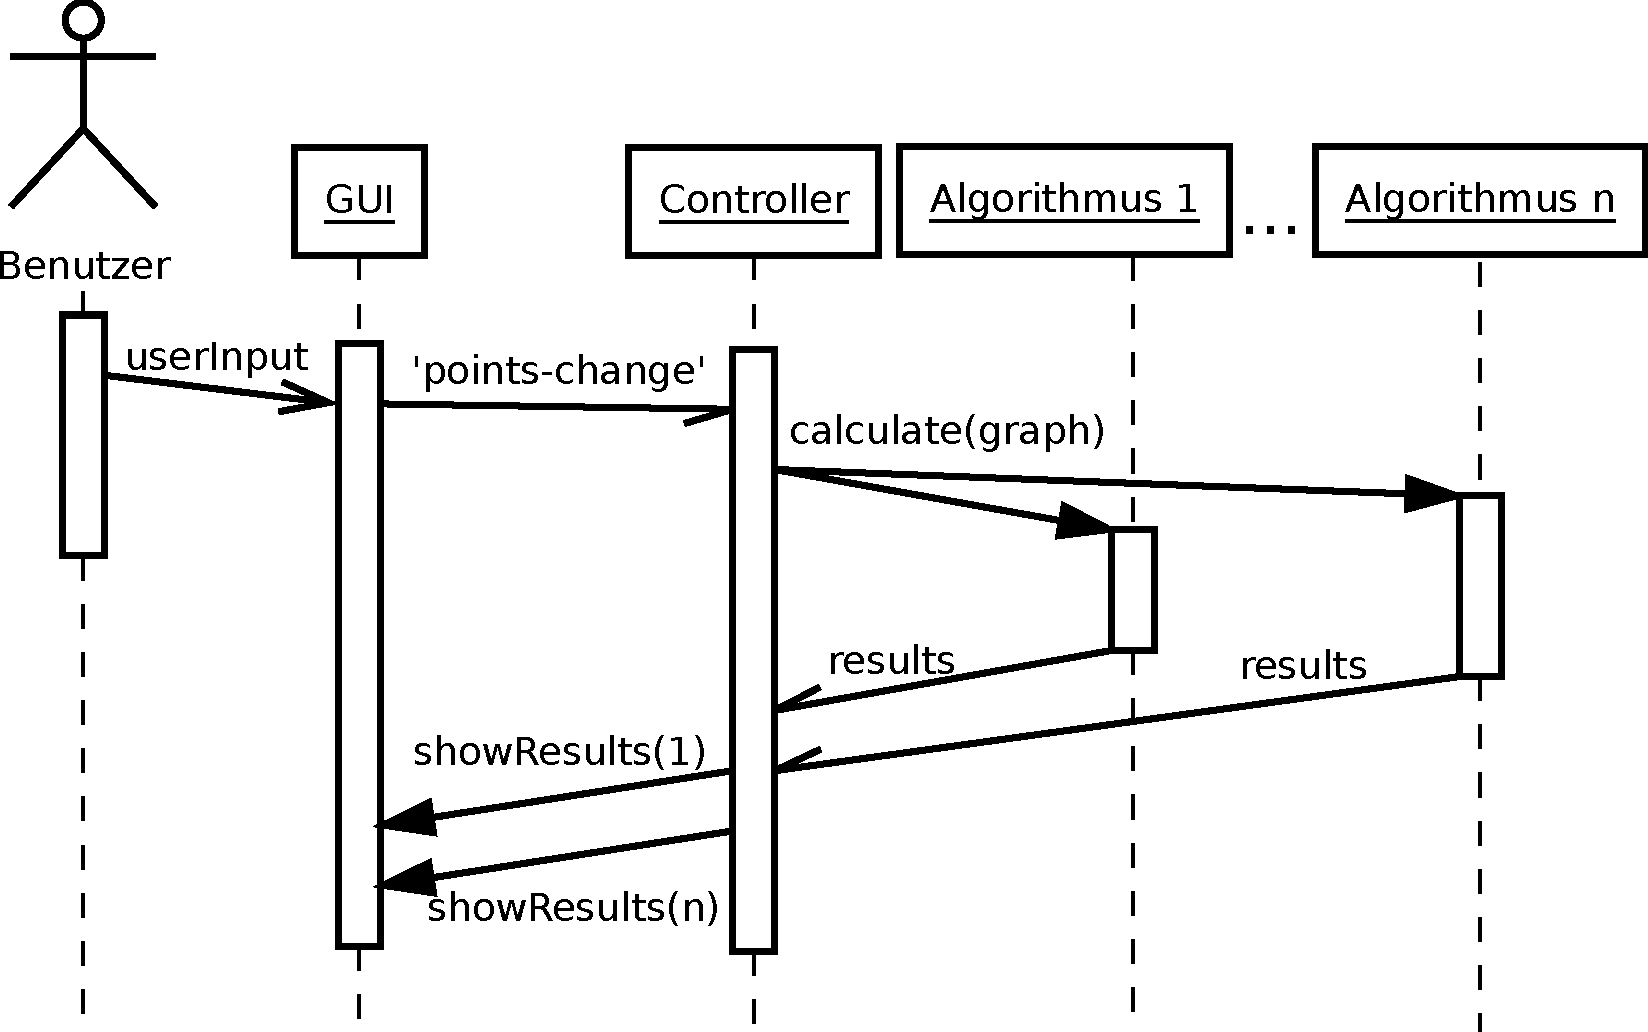
\includegraphics[width=0.5\textwidth]{Bilder/SequenceArchitecture}
\\\\
Hierbei stellen \texttt{'points-change'} und \texttt{results} Nachrichten dar, die Daten enthalten dar. \texttt{calculate(...)} und \texttt{showResults(...)} hingegen sind Methodenaufrufe der jeweiligen Objekte.
Es gibt drei Klassen von Akteuren: \emph{Webworker}, den zentralen \emph{Controller} und die \emph{GUI}, die grafische Benutzerschnittstelle.

\subsection{Webworker}
Um aus Benuztersicht die Ansprechbarkeit der Anwendung zu optimieren, haben wir uns dafür entschieden, die Berechnung der Algorithmen in Webworker auszulagern. Webworker ermöglichen es, in Javascript parallele Berechnungen ausführen zu lassen. So finden diese Berechnungen im Hintergrund statt, während die GUI weiterhin ansprechbar bleibt.
Beim Erstellen eines Webworkers wird ihm der auszuführende Code in Form eines Pfades zu einem Skript übergeben.
Da ein Webworker vom Hauptthread abgeschottet läuft und seinen eigenen Namensraum für Variablen besitzt, erfolgt jegliche Kommunikation über Nachrichten, welche neben Text auch ganze Objekte enthalten können.
Auf Anfrage wendet ein Webworker den im Skript enthaltenen Algorithmus an und sendet seine Ergebnisse zurück an den Controller. Die Anfrage besteht aus einer Nachricht, welche ein Graphobjekt und einen Namen enthält.

\subsection{Controller}
Der Controller(\emph{AlgLageController.js} ist einerseits dafür zuständig, die Algorithmen aufzurufen, andererseits um eine Brücke zwischen GUI und den Webworkern zu bauen, also Ergebnisse weiterzuleiten und Benutzereingaben zu verarbeiten. 
Ursprünglich sollte der Status der Anwendung lediglich im Controller gespeichert sein, allerdings wurde auch hier aus Gründen der Benutzbarkeit ein Teil des Status in die GUI ausgelagert.
Beim Erstellen eines Controllerobjektes wird ein GUIobjekt übergeben, um dem Controller direkten Zugriff auf Elemente und Methoden der GUI zu ermöglichen.
Im Gegensatz dazu funktioniert die Kommunikation mit den Workern asynchron über Nachrichten. Der Controller meldet sich mit \texttt{\$.subscribe('points-change', ...)} über jQuery beim Event \texttt{points-change} an. Dieses Event wird von der GUI gefeuert und zwar immer dann, wenn Punkte verschoben wurden. Da der eigentliche Koordinatenstatus der Punkte des Graphen in der GUI gespeichert ist, muss der Controller seinen internen Graphen mit den neuen Punkten der GUI updaten (\texttt{graph.points = gui.getPoints()}). Dann wird mit \texttt{calculateAlgos()} die Neuberechnung der Algorithmen gestartet.
Die Antworten der Worker werden in \texttt{handleResponse(event)} behandelt. Beim Hinzufügen eines Algorithmus wird das Ereignis, dass der Worker eine Nachricht postet mit dieser Methode verknüpft (\texttt{worker.onmessage = function(event) \{handleResponse(event);\}}) wobei \texttt{event} das Antwortobjekt darstellt.
Die Behandlung der Antwort beschränkt sich auf das Weiterleiten der in der Antwort enthaltenen Daten (\texttt{name}, \texttt{score}, \texttt{info}, \texttt{annots}) an die GUI.

\subsubsection{Graphen}
Um dem Controller einen neuen Graph zu übergeben kann entweder direkt ein Graph mit \texttt{setGraph(graph)} übergeben werden, welcher dann sofort geladen wird, oder man fügt ein neues \emph{Level} mit \texttt{addLevel(name, graph)} hinzu, wodurch der Graph unter dem übergebenen Namen im Controller abgespeichert wird. Mit \texttt{loadLevel(name)} wird ein vorher unter \emph{name} abgespeicherter Graph in die Ansicht geladen.

\subsubsection{Algorithmen}
Algorithmen müssen in einer Datei als Skript abgelegt sein, um mit \texttt{addAlgo(name, path)} dem Controller hinzugefügt werden zu können. Beim Hinzufügen eines Algorithmus wird ein neuer Webworker erstellt und eine Referenz auf ihn in einer Tabelle \emph{algos} abgelegt. Zusätzlich wird eine Farbe für die Anzeige der Ergebnisse des Algorithmus gesetzt und das \emph{ready}-Attribut des Algorithmus auf \emph{true} gesetzt (das bedeutet, dass der dem Algorithmus zugehörige Webworker gerade nicht beschäftigt ist). Zuletzt wird mit \texttt{gui.initAlgoBox(name, color)} in der GUI eine neue Box für die Anzeige der Ergebnisse des Algorithmus eingefügt.
Die Methode \texttt{calculateAlgos()} iteriert über alle mit \texttt{addAlgo(..)} hinzugefügten Algorithmen und sendet eine Neuberechnungsaufforderung an diejenigen Webworker, die nicht schon neuberechnen und auch in der GUI vom Benutzer als sichtbar eingestellt wurden.

\subsection{GUI}
\subsubsection{Aufbau}
Die GUI ist die Brücke zwischen Controller und Benutzer. Sie nimmt Benutzereingaben entgegen und gibt Statusinformationen des Programms graphisch aus. Die Darstellung der Graphen wird durch Einbindung von JSXGraph verwirklicht. JSXGraph stellt Werkzeuge zur Anzeige, Modifikation und Verwaltung von graphischen Objekten zur Verfügung. Neben der Grafikanzeige übernimmt die GUI auch die Anzeige von Textinformationen (wie z.B. den Score) und von Optionsmenüs (die Menüs selbst werden von Bootstrap erzeugt).
Die GUI erhält über \texttt{initGraph(graph)} eine Referenz auf den Graphen des Controllers.
Um die eigentliche Anzeige und Interaktivität der Punkte kümmert sich JSXGraph. Beim Initialisieren eines neuen Graphen wird \texttt{drawGraph(graph)} aufgerufen, welches die Punkte aus dem Graph Objekt liest und das \texttt{board} (also den JSXGraph Anzeigebereich) mit den entsprechenden graphischen Objekten füllt. Dabei werden an die erzeugten Objekte Eventhandler angebracht, die beim Eintreten einer Benuztereingabe (also dem Klicken und Verziehen von Objekten) an den Controller mit \texttt{\$.publish('points-change')} signalisieren, dass sich der Zustand des Graphen verändert hat. Dieser wird daraufhin mit der Methode \texttt{getPoints()} der GUI die aktuellen Koordinaten abfragen und sie an die Webworker weiterleiten.

\subsubsection{Methoden}
Hier werden die wichtigsten Methoden der GUI dokumentiert.
    \subparagraph{\texttt{initGraph(graph)}} 
    Zum Hinzufügen der Referenz auf den Graph des Controllers. Darüberhinaus wird hierüber der Bestwert initialisiert und der Graph gezeichnet.
    \subparagraph{\texttt{getPoints()}} 
    Simpler getter für die Punkte des Graphen.
    \subparagraph{\texttt{setPoints(points)}} 
    Hiermit werden die Punkte eines bereits initialisierten Graphen entsprechend der übergebenen Punktkoordinaten neu angeordnet. Die Struktur (also die Kanten) des Graphen bleibt bestehen.
    \subparagraph{\texttt{drawGraph()}} 
    Die Punkte und Kanten des \texttt{graph} werden dem JSXBoard hinzugefügt. Referenzen auf die Objekte liegen in \texttt{boardPoints} und \texttt{boardEdges}. Bei jedem Aufruf von \texttt{drawGraph()} werden die bisher in diesen Arrays enthaltenen Objekte vom \texttt{board} gelöscht und neu erstellt. Das Aufrufen dieser Methode ist nur einmal nach dem Initalisieren des Graphens notwendig, um die weitere Anzeige kümmert sich das JSXGraph Framework. Jedem graphischen Objekt wird ein Eventhandler hinzugefügt, der mit einem Timer verknüpft, bei Mausklicks das Event \texttt{'points-change'} in der Frequenz des Timers feuert. Hier geschieht auch die Bereichsabfrage, die das Verschieben der Punkte und Strecken auf einen bestimmten Rahmen (den Bereich des Rechtecks zwischen (0,0) und (\texttt{settings.maxX}, \texttt{settings.maxY}) ) einschränkt.
    Der Eventhandler der Kanten führt zusätzlich ein \texttt{Edge.reload()} auf der verschobenen Kante und allen inzidenten Kanten aus.
    \subparagraph{\texttt{overdraw(object, algoName, color)}} 
    Dasselbe wie \texttt{draw(...)} nur mit einem vorherigen Löschen aller Annotationen des jeweiligen Algorithmus.
    \subparagraph{\texttt{draw(object, algoName, color)}} 
    Hiermit können unabhängig vom Graphen Annotations gezeichnet werden. Die Annotations werden in eine eigene, von \texttt{algoName} abhängige Lage gezeichnet. \texttt{obj} muss dabei ein Annotations Objekt sein.
    \subparagraph{\texttt{eraseAllAnnotations()}} 
    Jegliche Annotations aller Algorithmen werden entfernt.
    \subparagraph{\texttt{eraseAnnotations(algoName)}} 
    Nur die Annotations, die zuvor unter \texttt{algoName} gezeichnet wurden, werden gelöscht.
    \subparagraph{\texttt{initAlgoBox(algoName, color)}} 
    Mit dieser Methode fügt man der Weboberfläche eine neue Anzeigebox für den Algorithmus mit Namen \texttt{algoName} hinzu und speichert für ihn eine Farbe ab, in der die Annotations angezeigt werden.
    \subparagraph{\texttt{setAlgoBoxLoading(algoName)}} 
    Hiermit wird die AlgoBox des zugehörigen Algorithmus mit Namen \texttt{algoName} mit einer Ladeanimation versehen. Diese Animation wird wieder entfernt mit \texttt{refreshAlgoBox(...)}.
    \subparagraph{\texttt{refreshAlgoBox(algoName, score, info, annots, color)}} 
    Wird benutzt, um die Ergebnisse eines Algorithmus anzuzeigen. Der Score (\texttt{score}), zusätzliche Informationen (\texttt{info}), Annotations (\texttt{annots}) werden geupdatet. Optional kann auch die eigentliche Farbe der Annotations eines Algorithmus hier überschrieben werden.
    Von der AlgoBox des zugehörigen Algorithmus mit Namen \texttt{algoName} wird die mit \texttt{setAlgoBoxLoading(...)} hinzugefügte Ladeanimation entfernt.
    \subparagraph{\texttt{addLevelToNav(levelName)}} 
    Dient zum Hinzufügen eines bereits mit \texttt{addLevel(levelName)} hinzugefügten Levels zur Weboberfläche im Dropdownmenü.
    \subparagraph{\texttt{changePageHeader(text)}} 
    Die Überschrift der Weboberfläche wird geändert.
    \subparagraph{\texttt{showHighscore(data)}} 
    Frede!
    \subparagraph{\texttt{clearHighscore()}} 
    Frede!
    \subparagraph{\texttt{setHighscoreVisibility(visible)}} 
    Frede!
    \subparagraph{\texttt{showGraph()}} 
    Der aktuell angezeigte Graph wird zu in der GraphTextArea genannten textarea serialisiert dargestellt.
    \subparagraph{\texttt{getGraph()}} 
    Der im Textfeld der Weboberfläche eingegebene Text wird mit \texttt{parseGraph(...)} eingelesen, als neues Level \textit{Custom '\#'} hinzugefügt und im Anzeigebereich angezeigt.
    \subparagraph{\texttt{isActive(algoName)}} 
    Gibt zurück, ob sich der Algorithmus mit Namen \texttt{algoName} gerade bei der Berechnung befindet.
    \subparagraph{\texttt{checkTmpBestval(val)}} 
    Speichert den aktuellen Graphen als bisher bestes Ergebnis ab, falls \texttt{val} den bisherigen bestwert übertrifft. Die Punkte des Graphen werden dabei in \texttt{bestPoints} abgelegt.

\subsection{Speicherung der Bestwerte}
In der Anwendung besteht die Möglichkeit einen erreichten Punktestand mit einem Formular in einer Bestenliste zu speichern. Dieser wird, wenn er zu den drei höchsten eines Levels gehört, danach in der Liste angezeigt. Zusätzlich wird zu einem Punktestand der Name des Benutzers angezeigt und es besteht die Möglichkeit, die Punkte auf die Positionen zu setzten, mit welchen der Punktestand erreicht wurde. Wie die hierfür benötigten Daten gespeichert und angezeigt werden soll nun genauer erläutert werden.\\
Um die Speicherung der Daten kümmert sich eine Datenbank, welche hierfür mit einer Tabelle versehen wurde. Diese enthält die Spalten „hid“, „levname“, „name“, „score“ und „points“. Hierbei ist „hid“ ein eindeutiger Schlüssel eines jeden Eintrags, „levname“ gibt an zu welchem Level ein Eintrag gehört, „name“ beinhaltet den Namen des Benutzers, „score“ entspricht dem erreichten Punktestand und in „points“ werden die Positionen der Punkte in einem String gespeichert. Da beim Anzeigen der Punktpositionen eines Bestwertes der Graph bereits geladen ist und sich die Reihenfolge der Punkte niemals ändert, genügt es nur die Positionen der jeweiligen Punkte zu speichern. Beim Klick auf den Pfeil werden dann die Punkte im Graph auf die gespeicherten Positionen verschoben.\\
Damit die Bestenliste auch funktionsfähig ist, wenn die Anwendung von einer lokalen Datei oder einem anderen Server ausgeführt wird und unabhängig von der Datenbank bleibt wurde zum Speichern der Daten eine Technik namens „JSON-P“ ausgewählt. Hiermit ist es möglich Daten von einem Server zu laden, der sich nicht auf der gleichen Domain befindet. Das ist mit aktuellem Javascript normalerweise nicht möglich.\\
Zum Laden der Punktestände wird eine PHP-Datei dynamisch wie folgt als Script in die HTML-Seite eingebunden:\\

\begin{lstlisting}
<script
 src="http://DB_SERVER/getscore.php">
</script>
\end{lstlisting}
Die Datei sieht dabei zum Beispiel wie folgt aus:

\newblock
\begin{lstlisting}
getResults('{
    "Haus vom Nikolaus": [
        {
            "name": "Wohoow",
            "score": "3.71269",
            "points": "[[7.34, 3.71], ...]"
        }, {
            "name": "Gut?",
            "score": "3.63707",
            "points": "[[0.18, 1.12], ...]"
        }, {
            "name": "mhh",
            "score": "2.58643",
            "points": "[[0,0], [11.64, 2.69], ...]"
        }');
    ]
}
\end{lstlisting}
\newblock
Durch das Einbinden der Datei als Script-Block wird der Inhalt danach vom Browser ausgeführt. Hier wird dann die Funktion „getResults“ mit den Daten aufgerufen. Diese befindet sich bereits von Beginn an in der Seite und kann somit die Daten entgegennehmen und verarbeiten.\\
Zum Speichern der Daten wird auf die gleiche Weise die folgende URL eingebunden:\\

\begin{lstlisting}
<script
 src="http://DB_SERVER/setscore.php?
   levname=Test&
   name=Name&
   score=0.02204&
   points=[[4,6],[12,4], ...]">
</script>
\end{lstlisting}
Der Server bekommt über die URL die Daten übergeben. Eine Rückantwort an die Anwendung wird hierbei nicht benötigt.\\
Somit ist es möglich die Bestenliste unabhängig vom Speicherort anzuzeigen, solange eine Internetverbindung besteht.


\section{Algorithmen}

\subsection{Test auf Kollinearität}
Ein sehr simples und essentielles Kriterium zur Überprüfung der allgemeinen Lage von Punkten ist der Test auf Kollinearität. Im speziellen ist hiermit der Fall von 3 oder mehr Punkten auf einer Geraden gemeint. Leider konnten wir dieses Problem von algorithmischer Seite nicht über eine Brute Force Lösung hinaus verbessern, wir vermuten allerdings, dass sich die Lösung bis auf hilfreiche Heuristiken und Verbesserungen der Implementierung auch nur schwer verbessern liesse. So müssen alle 3-Untermengen der Punktmenge gesondert auf Kollinearität überprüft werden, die dafür im wesentlichen benötigte Funktion ist \lststyle{e.contains(pt)} (siehe Kantenfunktionen). Um Ungenauigkeiten zu vermeiden wurde \lststyle{e} aus den beiden am weitesten auseinander liegenden Punkten generiert, \lststyle{pt} ist somit der dritte Punkt.  
\subsection{Berechnung der Schnittpunkte}
Ein wichtiger Algorithmus ist der zur Bestimmung von Schnittpunkten von Kanten, da unser primärer Algorithmus zur Bewertung der Punktlage ~-- der Algorithmus zur Bestimmung der kürzesten Distanz von einem Punkt zu einer Kante ~-- auf diesen fusst.  
\subsection{Punkte befinden sich auf Kreis}
Ein weiteres Kriterium für die Bewertung der allgemeinen Lage von Punkten, welches im Rahmen dieses Projekts umgesetzt wurde, besteht darin zu berechnen, ob mehr als drei Punkte auf einem Kreis liegen. Da drei Punkte immer auf einem Kreis liegen ist hierdurch noch keine Besonderheit gegeben, was die Lage der Punkte im Koordinatensystem anbelangt. Da mehr als drei Punkte jedoch nicht immer zwingend auf einem Kreis liegen müssen, kann eine solche Anordnung so als Sonderfall betrachtet werden, die einer allgemeinen Lage der Punkte wiederspricht.\\
Um dieses Kriterium zu betrachten wurde kein mathematischer Ansatz gewählt, der auf der Berechnung von Kreisgleichungen basiert, sondern eher ein grafischer. Dieser soll im Folgenden genauer erläutert werden.\\
Um zu untersuchen, ob verschiedene Punkte auf einem Kreis liegen könnte ein Ansatz darin bestehen viele Kreise mit verschiedenen Radien und Positionen durchzuprobieren und jedes Mal zu zählen, wie viele Punkte sich auf einem solchen Kreis befinden. Dabei würde es jedoch eine große Anzahl an Kreisen geben, auf denen sich gar keine der Punkte befinden und die somit umsonst betrachtet werden würden.\\
Aus diesem Grund wurde hier der genau umgekehrte Ansatz gewählt die Kreise mit verschiedenen Radien um die Punkte selber zu ziehen und dann zu schauen, wie viele der Kreise sich im selben Schnittpunkt treffen. Gibt es einen Schnittpunkt in dem sich zum Beispiel vier Kreise treffen, dann bedeutet dies, dass sich um diesen Schnittpunkt ein Kreis mit dem gleichen Radius ziehen lässt, der dann wiederum genau diese vier Punkte schneidet.
 
\begin{figure}[h]
\centering
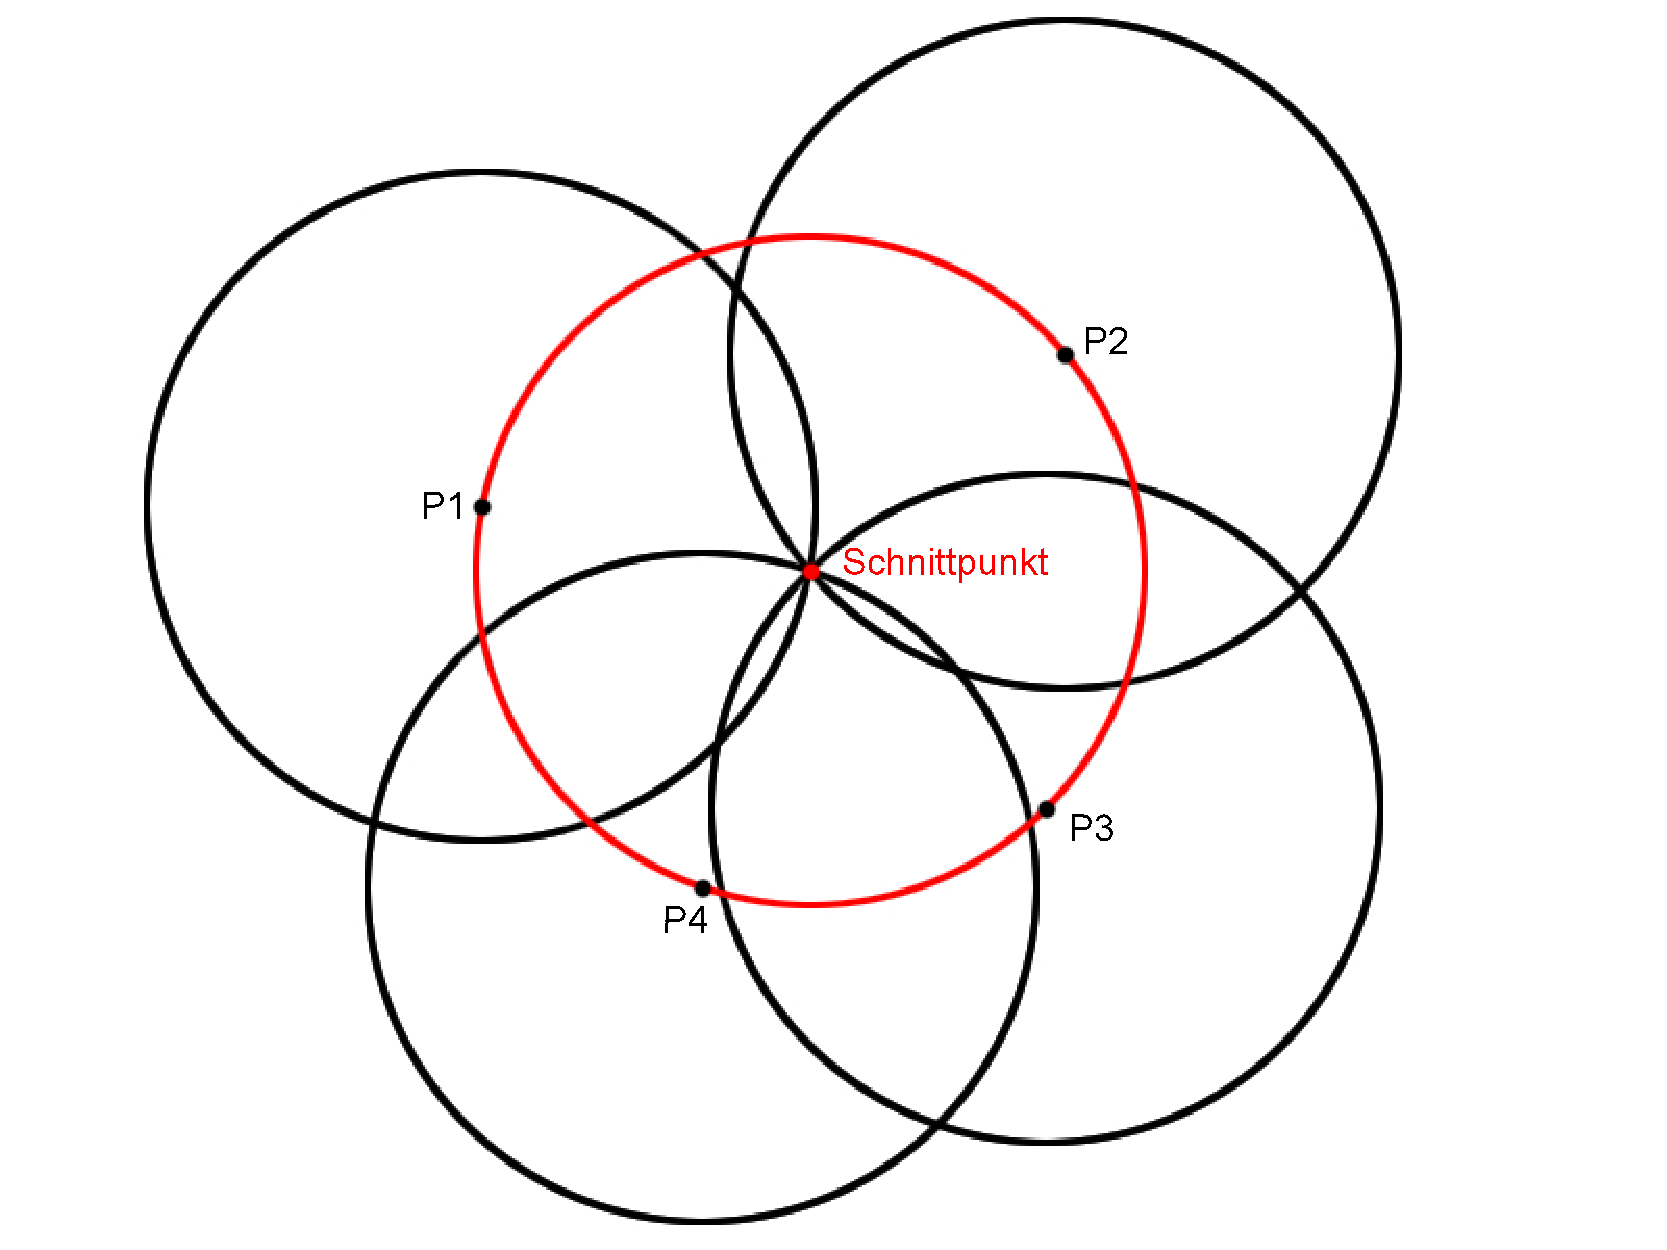
\includegraphics[width=0.5\textwidth]{Bilder/kreise}
\caption{Umgekehrte Heransgehensweise um Punkte auf Kreis zu finden}
\label{img:kreise}
\end{figure}

Es muss somit also nur geschaut werden, ob es bei verschiedenen Radien Schnittpunkte gibt, in denen sich mehr als drei Kreise treffen. Die jeweiligen Schnittpunkte und Radien werden dann vom Algorithmus zurückgegeben und grafisch dargestellt.\\
Der Algorithmus erstellt hierfür zunächst ein Array, welches von den Proportionen der Größe des Sichtbereiches entspricht. Die Kreise werden dann diskretisiert um die jeweiligen Punkte in das Array übertragen. Die Punkte sind hierbei vorher ebenfalls diskretisiert und auf die Größe des Arrays angepasst worden.\\
Die Kreise werden nicht einfach nur „gezeichnet“, sondern es wird im Array, welches vom Typ Integer ist, an jeder Position an der sich der Kreis befindet um Eins inkrementiert. Ein Kreis ist also zunächst durch eine diskrete Anordnung von Einsen im Array dargestellt. Wird nun ein Kreis um einen weiteren Punkt eingezeichnet, der mit dem vorherigen Kreis einen Schnittpunkt hat, so ergibt sich an dem Schnittpunkt im Array ein Wert von Zwei. Sind alle Kreise eingezeichnet worden muss so am Ende nur im Array nach allen Werten gesucht werden, die größer als drei sind. Hier befindet sich ein Schnittpunkt von mehr als drei Kreisen mit dem betrachteten Radius.

\begin{figure}[h]
\centering
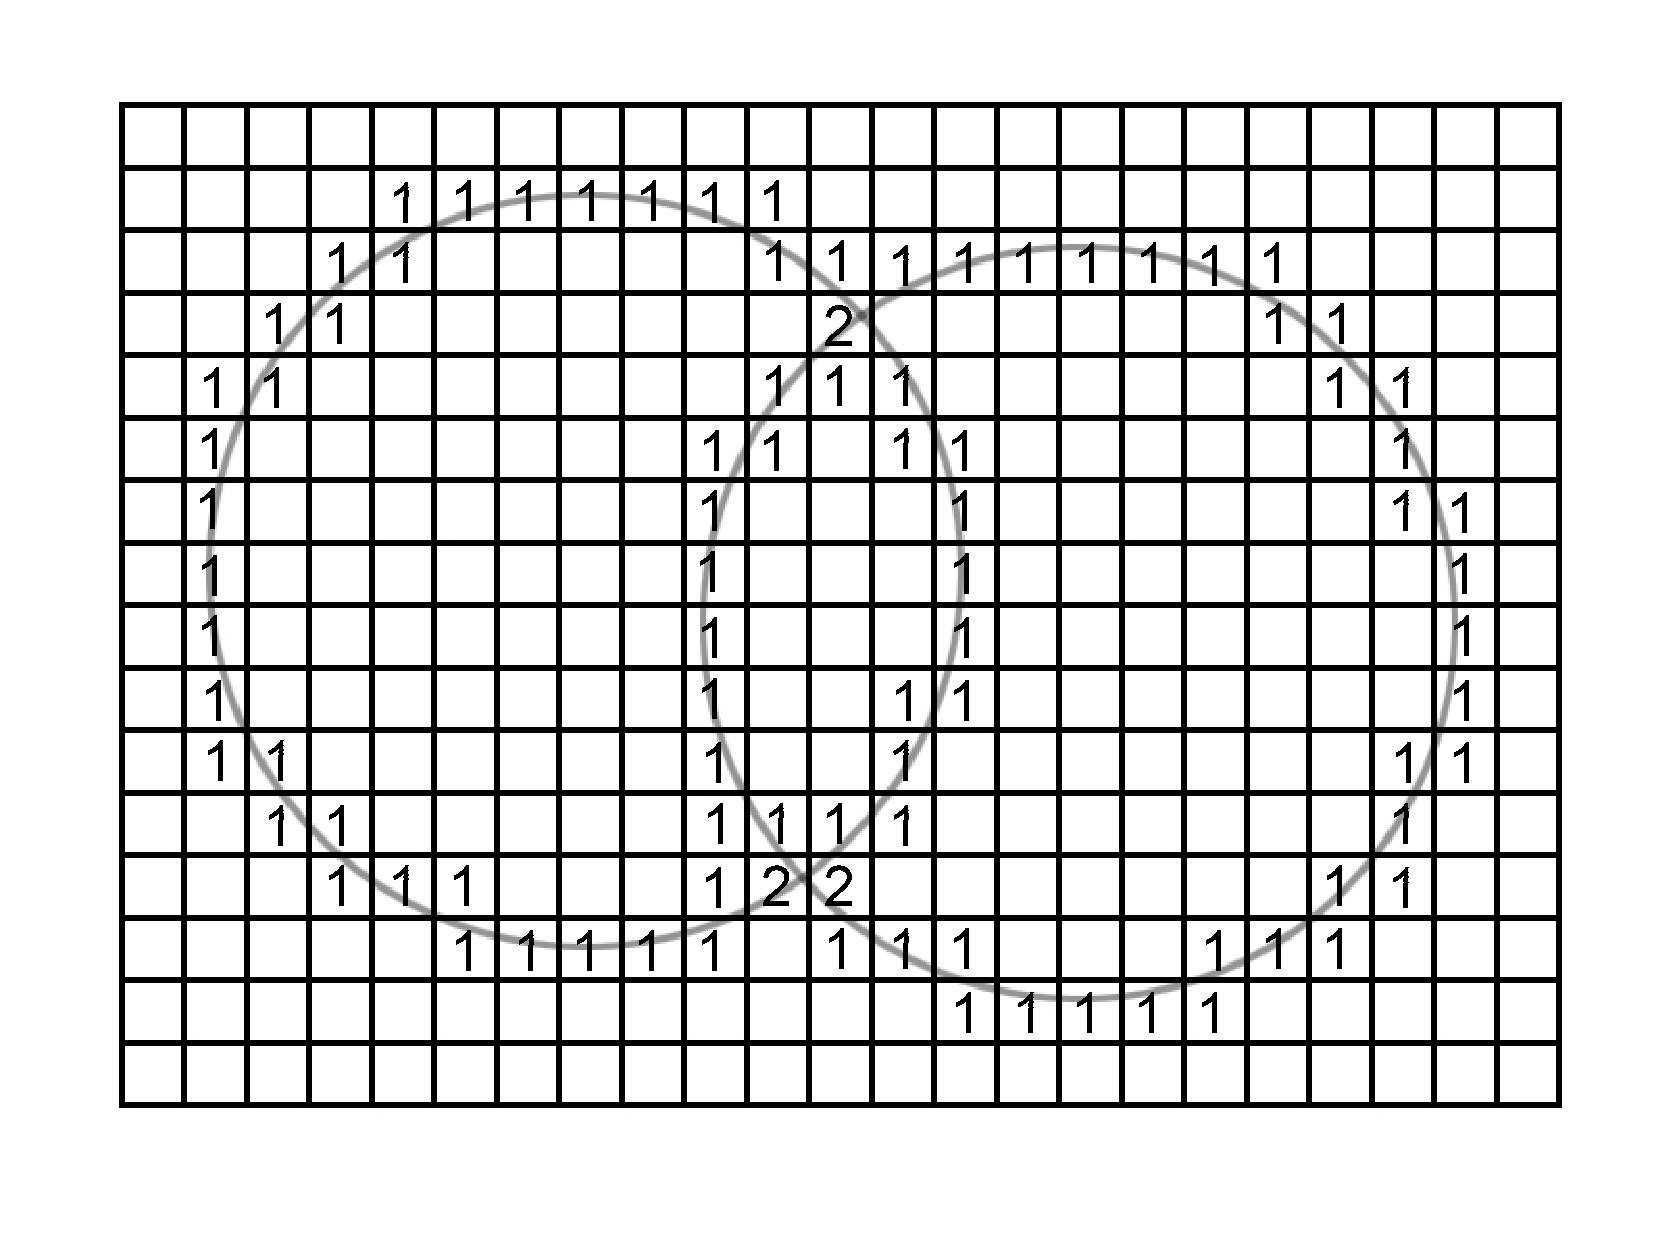
\includegraphics[width=0.5\textwidth]{Bilder/diskret}
\caption{Überscheidung von zwei diskretisierten Kreisen im Array}
\label{img:diskret}
\end{figure}

Die Genauigkeit mit der die Punkte auf einem Kreis liegen lassen sich im Algorithmus über die Größe des Arrays bestimmen. Je größer das Array, desto genauer liegen die Punkte am Ende auf dem Kreis. Hier wurde eine relativ kleine Größe des Array gewählt, sodass Punkte auch dann als auf dem Kreis liegend bewertet werden, wenn sie sich etwas daneben befinden.\\
Als Score ließe sich hier der Abstand der Punkte zu einer möglichen Lage auf einem Kreis angeben. In diesem Projekt wurde jedoch nur überprüft, ob sich mehr als drei Punkte mit einer gewissen Unschärfe auf einem Kreis befinden.












\end{document}
